% Passover Seder Liturgy
\documentclass[10pt,oneside,footinclude=true,headinclude=true]{scrbook} % KOMA-Script book
\usepackage[LHE,T1]{fontenc}
\usepackage[linedheaders,manychapters,parts]{classicthesis}
\usepackage[paperheight=8.5in,paperwidth=5.5in,margin=0.8in]{geometry}
\usepackage{graphicx}

\usepackage[english]{babel}

\usepackage{paracol}
\usepackage{transparent}
\usepackage{cancel}
\usepackage{tikz}
\usetikzlibrary{calc}

%\usepackage{palatino}

% Better underlining.
\usepackage{ulem}
\usepackage{contour}
\renewcommand{\ULdepth}{1.3pt}
\contourlength{0.7pt}
\newcommand{\textul}[1]{%
  \uline{\phantom{#1}}%
  \llap{\contour{white}{#1}}%
}

% Helper functions.
\newcommand\recitwidth{7.7cm}
\newcommand\oldrecite[2]{ \ifthenelse{\equal{#1}{All}} {\textbf{#1} : & \textbf{\small #2}} {#1 : & \small #2} }

\newcommand\recitecol[2]{
	\small{
		\begin{paracol}{2}
		\columnratio{0.15,0.85}
			\begin{leftcolumn}
			#1 :
			\end{leftcolumn}
			\begin{rightcolumn}
			\noindent #2
			\end{rightcolumn}
		\end{paracol}
	}
}
\newcommand\recite[2]{
	\ifthenelse{\equal{#1}{All}}
	{\textbf{\recitecol{#1}{#2}}}
	{\recitecol{#1}{#2}}
}

\newcommand\quot[1]{
	\begin{quote}\textit{\small#1}\end{quote}
}

\newcommand\pagequot[1]{
	\newpage
	\clearscrheadfoot
	%\vspace*{\fill}
	\vspace*{\stretch{2}}
	\begin{center}
	\begin{minipage}[c]{8cm}
		#1
	\end{minipage}
	\end{center}
	%\vspace*{\fill}
	\vspace*{\stretch{3}}
}

\newcommand{\positionbox}[3]{
	\begin{tikzpicture}
		\node[inner sep=0pt] at ($(current page.north west) + (#1,-#2)$)
			{\transparent{0.1}\includegraphics[width=2in]{#3}};
	\end{tikzpicture}
}

\newcommand{\drawimage}[4]{
	\makebox[0pt][s]{
		\raisebox{#1}[0pt][0pt]{
			\transparent{#2}\includegraphics[width=#3]{#4}
		}
	}
}

\begin{document}

%---------------------------------------------------------------------------------------
%	TITLE PAGE
%---------------------------------------------------------------------------------------
\begin{titlepage}
\begin{center}
\large \hfill \vfill

\begingroup
\color{NavyBlue}\spacedallcaps{The Jusman Family} \\
\bigskip
\color{NavyBlue}\spacedallcaps{\huge{Passover Liturgy}} \\ %Title
\bigskip
\endgroup

\bigskip\bigskip
\bigskip\bigskip
\bigskip\bigskip
\bigskip
%\spacedlowsmallcaps{J.Jusman}
%\vfill
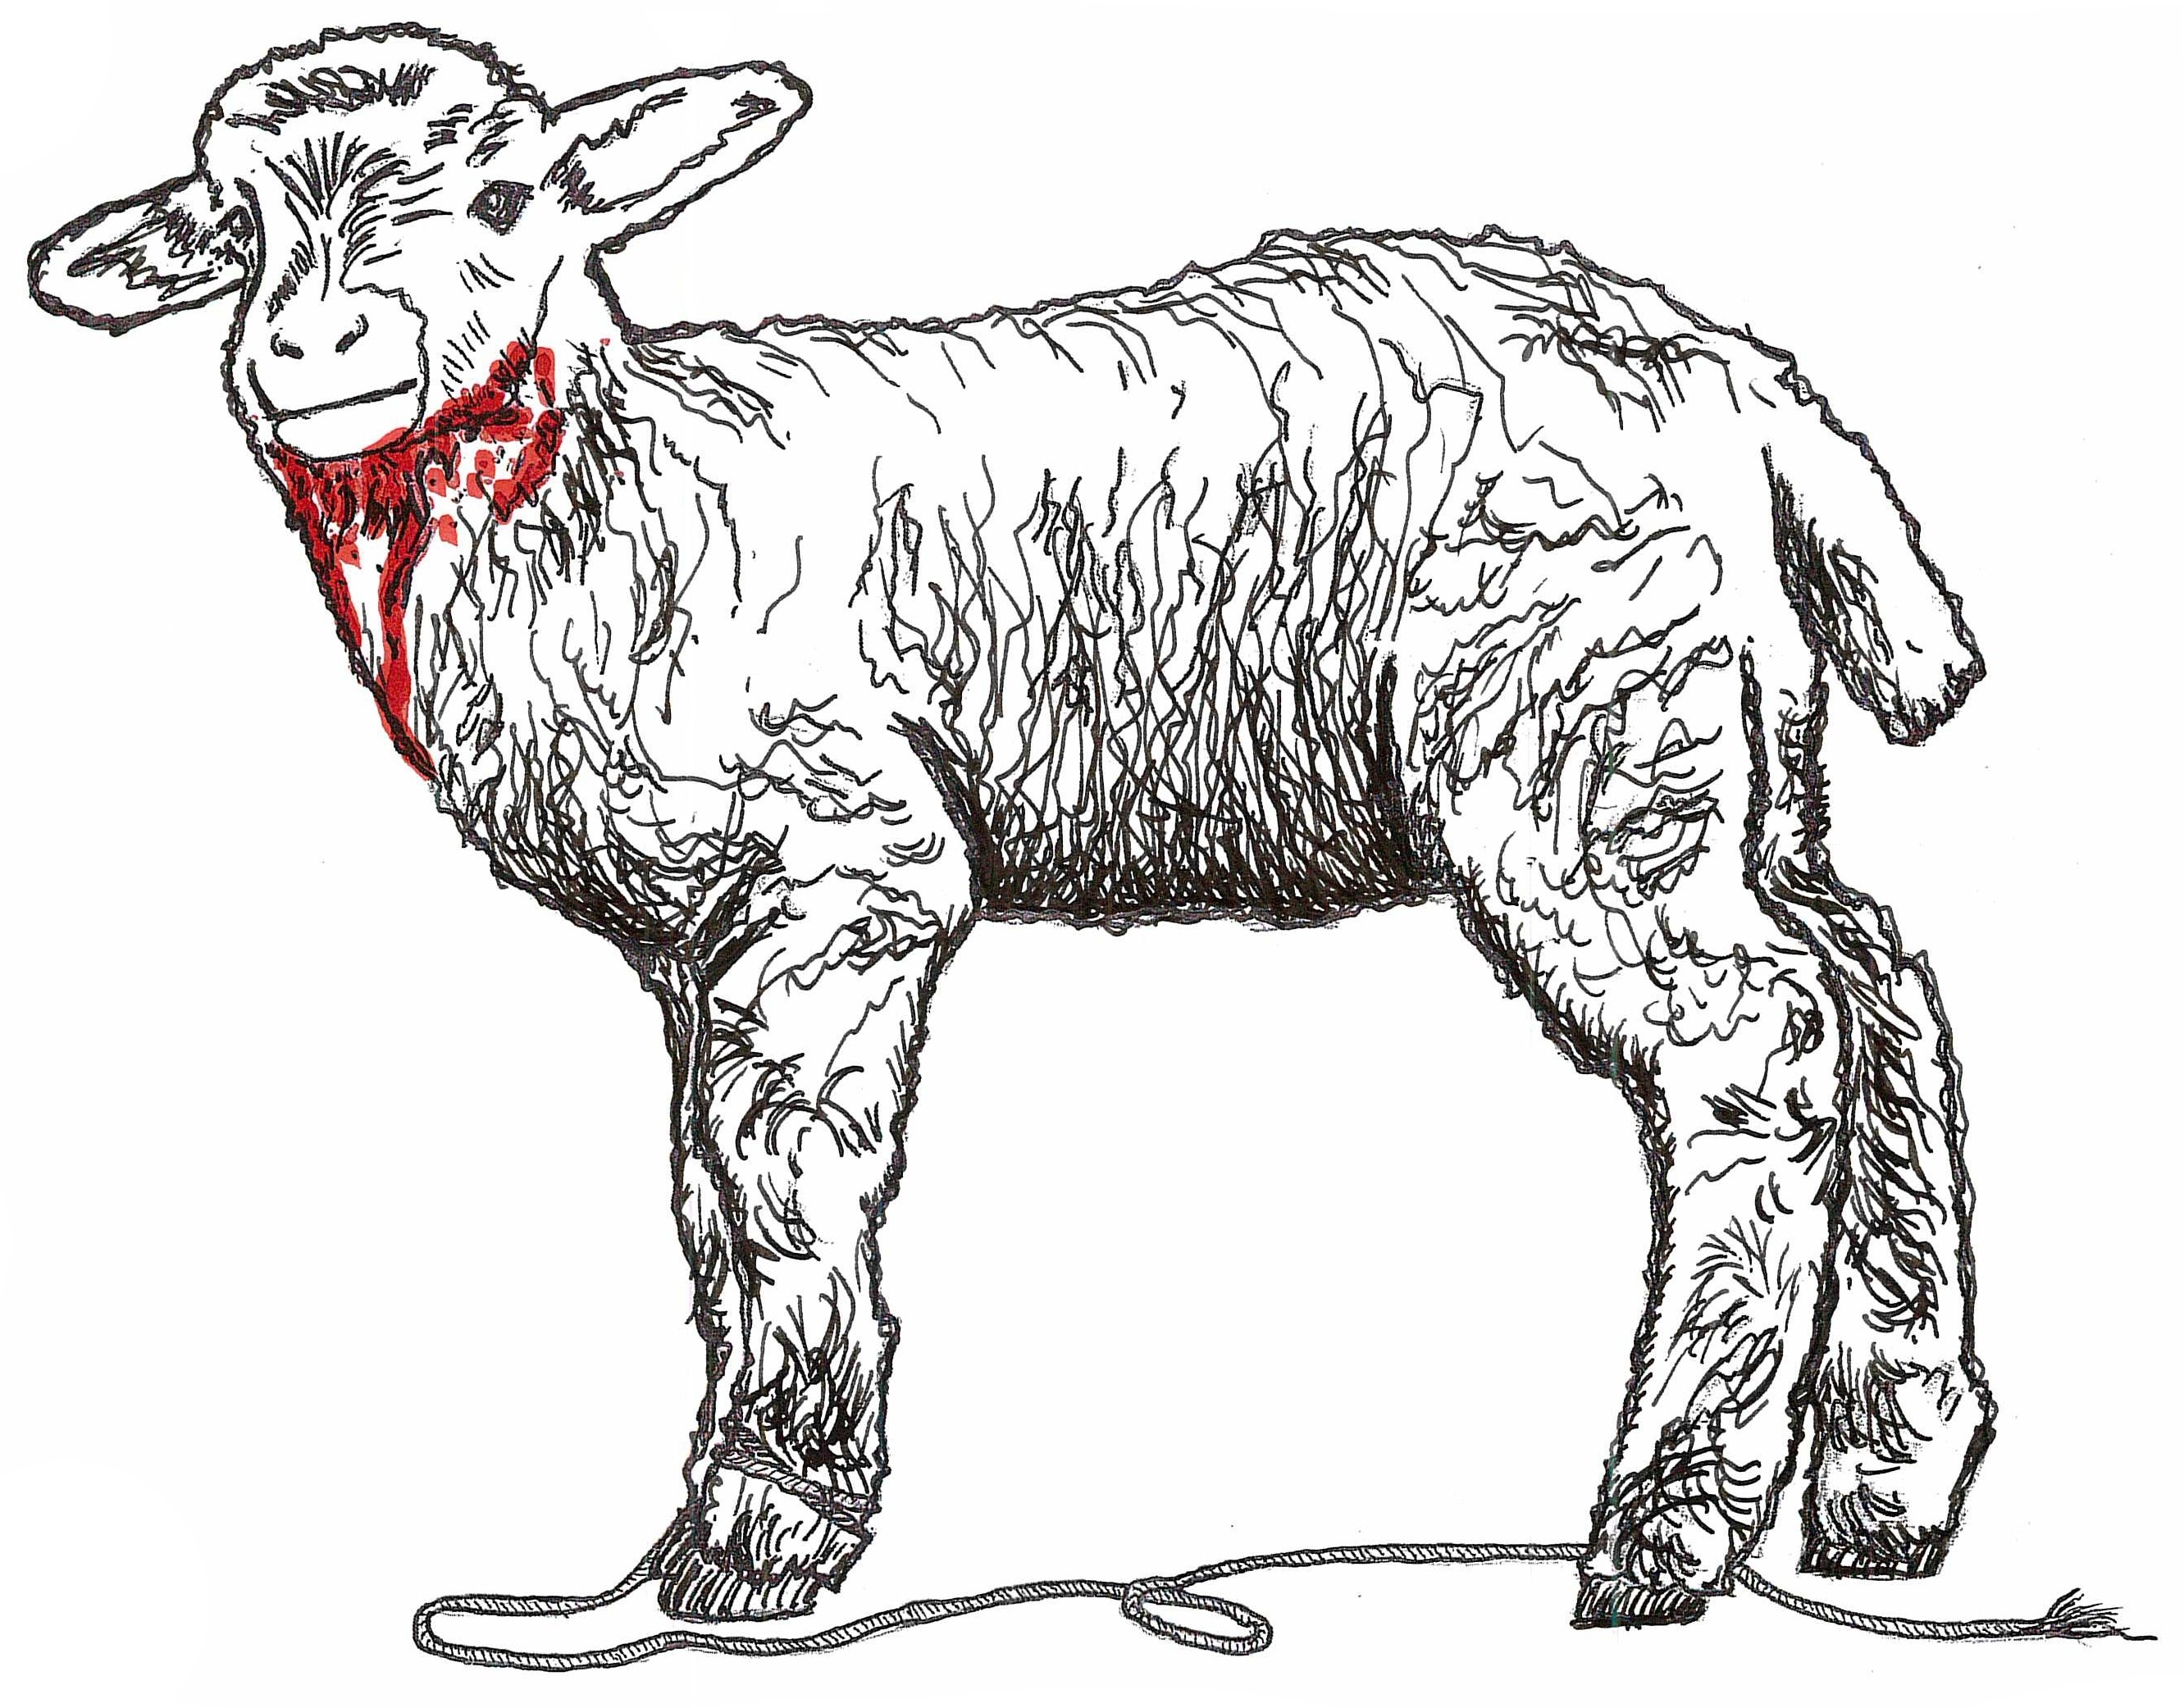
\includegraphics[width=4cm]{lamb3nooval} \\
%\vfill
\bigskip
\bigskip\bigskip
\bigskip\bigskip
\bigskip\bigskip

\textit{...And when I see the blood, I will pass over you...} \\ \medskip % Subtitle

April 2019\ -- version 1.5 % Time and version

\vfill
\end{center}
\end{titlepage}
    
%\newpage
%\clearscrheadfoot
%\null

%---------------------------------------------------------------------------------------

\pagequot{
\centering
\textit{
Let not the foreigner who has joined himself to the LORD
say, "The LORD will surely separate me from his people"...\\
\smallskip
...And the foreigners who join themselves to the LORD,\\
    to minister to him, to love the name of the LORD,\\
    and to be his servants,\\
everyone who keeps the Sabbath and does not profane it,\\
    and holds fast my covenant--\\
these I will bring to my holy mountain,\\
    and make them joyful in my house of prayer;\\
their burnt offerings and their sacrifices\\
    will be accepted on my altar;\\
for my house shall be called a house of prayer\\
    for all peoples.\\
}
\bigskip
\spacedlowsmallcaps{Isaiah 56:3, 6-7}
}
%---------------------------------------------------------------------------------------
%	TOC
%---------------------------------------------------------------------------------------
\tableofcontents 
\cleardoublepage % use \cleardoublepage here to avoid problems with pdfbookmark


%---------------------------------------------------------------------------------------
%	INTRODUCTION
%---------------------------------------------------------------------------------------
\setcounter{chapter}{-1}
\chapter{Introduction}

Why?\\
\\
Why we Chinese/Indonesian people be doing these weird Jewish people things?\\
\\
A couple of reasons:
\begin{enumerate}
	\item{
		Because the Passover traditions are beautiful and they point to our savior Jesus ("Yeshua").
		\quot{Behold, the Lamb of God, who takes away the sin of the world! (John 1:29)}
	}
	\item{
		Because Yeshua himself celebrated Passover and followed a Jewish liturgy.
		\quot{They are Israelites, and to them belong the adoption, the glory, the covenants, the giving of the law, the worship, and the promises. (Romans 9:4)}
		\quot{So Yeshua sent Peter and John, saying, "Go and prepare the Passover for us, that we may eat it." (Luke 22:8)}
	}
	\item{
		Because what we call "communion" at church is actually a couple of elements from the Passover dinner.
		\quot{For I received from the Lord what I also delivered to you, that the Lord Yeshua on the night when he was betrayed took bread, and when he had given thanks, he broke it, and said, "This is my body which is for you. Do this in remembrance of me." In the same way also he took the cup, after supper, saying, "This cup is the new covenant in my blood. Do this, as often as you drink it, in remembrance of me." (1 Corinthians 11:23-25)}
	}
	\item{
		Because the Passover Exodus was experienced by non-Jewish peoples also, aka Gentiles like us.
		\quot{And the people of Israel journeyed from Rameses to Succoth, about six hundred thousand men on foot, besides women and children. A mixed multitude also went up with them... (Exodus 12:37-38)}
	}
		\quot{Then whoever feared the word of the LORD among the servants of Pharaoh hurried his slaves and his livestock into the houses, but whoever did not pay attention to the word of the LORD left his slaves and his livestock in the field. (Exodus 9:20-21)}
	\item{
		Because it is cool and weird even to the Jewish people.
		\quot{And when your children say to you, "What do you mean by this service?" you shall say, "It is the sacrifice of the LORD's Passover, for he passed over the houses of the people of Israel in Egypt, when he struck the Egyptians but spared our houses." (Exodus 12:26-27)}
		\quot{When your son asks you in time to come, "What is the meaning of the testimonies and the statutes and the rules that the LORD our God has commanded you?" then you shall say to your son, "We were Pharaoh's slaves in Egypt. And the LORD brought us out of Egypt with a mighty hand..." (Deuteronomy 6:20-21)}
	}
	\item{
		Because the Passover is the first proper commandment of God to his people, even before the Ten Commandments.
		\quot{This day shall be for you a memorial day, and you shall keep it as a feast to the LORD; throughout your generations, as a statute forever, you shall keep it as a feast. (Exodus 12:14)}
	}
	\item{
		Because it's fun, and it's a feast, and we like to eat! Plus, this feast celebrates not only 1 Exodus, but 2 Exoduses, where God saved his people from bondage by a mighty hand and an outstretched arm.
		\quot{And behold, two men were talking with him (Yeshua), Moses (Moshe) and Elijah (Eliyahu), who appeared in glory and spoke of his departure (exodus), which he was about to accomplish at Jerusalem. (Luke 9:30-31)}
	}
\end{enumerate}


\section{The Feast}
The Passover is the most commonly celebrated Jewish feast. The liturgy for the meal is called the "Seder" (the "Order"), but the feast itself is called "Pesach." It is the meal of Yeshua's "Last Supper" with his disciples.

\quot{And when the hour came, he reclined at table, and the apostles with him. And he said to them, "I have earnestly desired to eat this Pesach with you before I suffer. For I tell you I will not eat it until it is fulfilled in the kingdom of God." (Luke 22:14-15)}


\section{The Rhyme}

The Seder liturgy is summarized in a nice little rhyme that spells out the order of the whole meal. Each of these little words signifies a step in the order.\\
\\
Qaddesh Urchatz, Karpas Yachatz\\
Maggid Rachtza, Motzi Mattza\\
Maror Korekh, Shulchan Orekh\\
Tzafun Barekh, Hallel Nirtza


\section{The Liturgy}

The liturgy is based on 4 cups of blessings, which correspond to God's 4 promises to his people while they were still slaves in Egypt, the house of bondage. There are 3 other promises there in the passage (Exodus 6:6-8) that the Jews somehow didn't include in their traditional liturgy, and I don't know why, but such is life :) Probably because 4 cups of wine are OK but 7 cups could get you drunk?? :) Anyway don't worry, I have included the other 3 promises somewhere in this booklet. We are doing a simplified liturgy, instead of a full-fledged one. Many items have been removed from the traditional Seder for reasons of time and my own ignorance. Sorry =)\\
\\
Items needed for the liturgy:
\begin{enumerate}
	\item{Two candles}
	\item{Roast lamb (The Jews today don't eat lamb at Pesach because the temple was destroyed in 70 AD. They only include a lamb bone for remembrance)}
	\item{Grape juice or wine}
	\item{Unleavened bread or Matzah}
	\item{A white cloth to wrap the unleavened bread}
	\item{A linen cloth/napkin to hide the Afikoman}
	\item{A water pitcher, a washing bowl or basin, a hand towel}
	\item{A green vegetable, e.g. celery or parsley: representing fertility and growth}
	\item{A bitter herb, e.g. endive, dandelion, horseradish: representing the bitterness of slavery}
	\item{A bowl of salt water: representing sweat and tears during slavery, also representing the Red Sea}
	\item{An extra cup and an extra chair: for Eliyahu (if you are Jewish), for Yeshua (if you are Christian)}
\end{enumerate}

\vspace{5mm}

To lead the liturgy, you need to be the firstborn male in your family, circumcised on the eighth day, from the clan of Judah, clean-shaven and completely bald Nahh... just kidding! :) Anyone can be the leader if s/he so desires.\\

I have included lots of Scriptures in the booklet. These are for reading out loud together, or quietly on your own. Up to you. Some of the Scriptures show the places in the Bible where a Seder word occurs in exactly the same form. And some Scriptures show the places in the Bible where it occurs for the first time.\\

\noindent Let's begin the liturgy.\\
\\
\small
Eldest Woman: Let the eldest woman in the house light up two candles. (Usually every Sabbath, the youngest female in the house lights up the candles. But for Pesach, it's the eldest woman.)\\

\columnratio{0.15,0.85}

%\newpage
%\clearscrheadfoot
%\null

%---------------------------------------------------------------------------------------
%	PART I
%---------------------------------------------------------------------------------------
\normalsize
\pagequot{
\centering
\textit{I am the LORD, and \textbf{I will bring you out} from under the burdens of the Egyptians, and \textbf{I will deliver you} from slavery to them, and \textbf{I will redeem you} with an outstretched arm and with great acts of judgment. \textbf{I will take you} to be my people,...}\\
\bigskip
\spacedlowsmallcaps{Exodus 6:6-8}
}

%---------------------------------------------------------------------------------------
\part{The First Cup: I Will Bring You Out}

\chapter{Qaddesh: Sanctify} 
%\drawimage{9mm}{0.1}{10cm}{qaddesh}

%\positionbox{2cm}{2cm}{qaddesh}
%\makebox[0pt][s]{%
%%  \raisebox{\totalheight}[0pt][0pt]{%
%  \raisebox{1cm}[0pt][0pt]{%
%    {\transparent{0.1}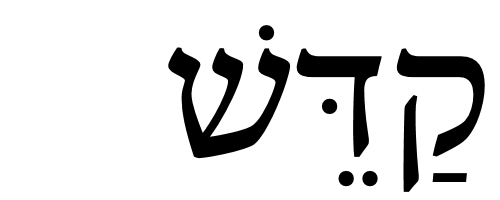
\includegraphics[width=10cm]{qaddesh}}
%}}%

\normalsize
Step \thechapter: Sanctifying the wine.\\
\\
The Qiddush ("Sanctification") is a Sabbath blessing recited over wine or grape juice. It's recited weekly to sanctify the Sabbath, but also on Jewish holidays. The Shehecheyanu ("Who has given us life") is a blessing recited during special occasions, e.g. the beginning of a holiday or feast.

\vspace{5mm}
\hrule
\vspace{5mm}

The Qiddush:\\

\recite{Leader}{And there was evening and there was morning, the sixth day. Thus the heavens and the earth were finished, and all the host of them. And on the seventh day God finished his work that he had done, and he rested on the seventh day from all his work that he had done. So God blessed the seventh day and sanctified it, because on it God rested from all his work that he had done in creation.}

\recite{All}{Blessed are you O LORD our God, king eternal, creator of the fruit of the vine.}

\recite{All}{[Pour a little wine for the person sitting to your left]}
\hfill

\recite{Leader}{Blessed are you O LORD our God, king eternal, who sanctified us with his commandments, and was pleased with us, and invested us with his holy Sabbath in love and favor, as a memorial of the Creation. For it is foremost among the holy festivals commemorating the exodus from Egypt. For you chose us and sanctified us, out of all the peoples, and you invested us with your holy Sabbath in love and favor. Blessed are you O LORD, who sanctifies the Sabbath.}

\recite{All}{Amen.}

\vspace{5mm}
\hrule
\vspace{5mm}

\normalsize
The Shehecheyanu:\\

\recite{Leader}{Blessed are you O LORD our God, king eternal, who has given us life and sustained us and brought us to this occasion.}

\recite{All}{Amen.}

\recite{All}{[Drink the first cup]}

\vspace{5mm}
\hrule
\vspace{5mm}

\quot{And God saw everything that he had made, and behold, it was very good. And there was evening and there was morning, the sixth day. Thus the heavens and the earth were finished, and all the host of them. And on the seventh day God finished his work that he had done, and he rested on the seventh day from all his work that he had done. So God blessed the seventh day and \textul{made it holy}, because on it God rested from all his work that he had done in creation. (Genesis 1:31-2:3)}

\quot{\textul{Consecrate (qaddesh)} to me all the firstborn. Whatever is the first to open the womb among the people of Israel, both of man and of beast, is mine. (Exodus 13:2)}

\quot{\textul{Sanctify} them in the truth; your word is truth. As you sent me into the world, so I have sent them into the world. And for their sake I \textul{sanctify} myself, that they also may be \textul{sanctified} in truth. (John 17:17-19)}

%---------------------------------------------------------------------------------------
\chapter{Urchatz: And Wash}
%\drawimage{9mm}{0.1}{10cm}{urchatz}
\normalsize
Step \thechapter: Washing the hands.\\
\\
The youngest child in the house carries a towel around the table and dries everyone's hands.

\vspace{5mm}
\hrule
\vspace{5mm}

\recite{All}{[Pour water over the hands of the person to your right]}
\vspace{3mm}
\recite{Child}{[Dries hands with towel]}

\vspace{5mm}
\hrule
\vspace{5mm}

\quot{Yeshua, knowing that the Father had given all things into his hands, and that he had come from God and was going back to God, rose from supper. He laid aside his outer garments, and taking a towel, tied it around his waist. Then he poured water into a basin and began to wash the disciples' feet and to wipe them with the towel that was wrapped around him.}

\quot{He came to Simon Peter (Shim`on Kefa), who said to him, "Lord, do you wash my feet?" Yeshua answered him, "What I am doing you do not understand now, but afterward you will understand." Kefa said to him, "You shall never wash my feet." Yeshua answered him, "If I do not wash you, you have no share with me." Shim`on Kefa said to him, "Lord, not my feet only but also my hands and my head!"}

\quot{Yeshua said to him, "The one who has bathed does not need to wash, except for his feet, but is completely clean. And you are clean, but not every one of you." For he knew who was to betray him; that was why he said, "Not all of you are clean." When he had washed their feet and put on his outer garments and resumed his place, he said to them, "Do you understand what I have done to you?.. (John 13:3-12)}

\quot{And the LORD appeared to him (Abraham) by the oaks of Mamre, as he sat at the door of his tent in the heat of the day. He lifted up his eyes and looked, and behold, three men were standing in front of him. When he saw them, he ran from the tent door to meet them and bowed himself to the earth and said,}

\quot{"O Lord, if I have found favor in your sight, do not pass by your servant. Let a little water be brought, and \textul{wash} your feet, and rest yourselves under the tree, while I bring a morsel of bread, that you may refresh yourselves, and after that you may pass on---since you have come to your servant." So they said, "Do as you have said." (Genesis 18:1-5)}

\quot{You shall also make a basin of bronze, with its stand of bronze, for \textul{washing (rachtza)}. You shall put it between the tent of meeting and the altar, and you shall put water in it (Exodus 30:18)}


%---------------------------------------------------------------------------------------
\chapter{Karpas: Vegetable}
%\drawimage{9mm}{0.1}{10cm}{karpas}
\normalsize
Step \thechapter: Eating vegetables dipped in the salt water.\\
\\
The green vegetable reminds us that it was springtime when the Exodus took place. It also represents growth and fertility of the Jewish people in Egypt. The salt water represents their sweat and tears during slavery, and also their crossing the Red Sea.

\vspace{5mm}
\hrule
\vspace{5mm}

\recite{All}{Blessed are you O LORD our God, king eternal, creator of the fruit of the earth. Amen.}

\recite{All}{[Dip the vegetable in the salt water. Don't forget to shake off some salt water drops, resembling tear drops]}

\recite{All}{[Eat the vegetable]}

\vspace{5mm}
\hrule
\vspace{5mm}

\quot{As for the one who is weak in faith, welcome him, but not to quarrel over opinions. One person believes he may eat anything, while the weak person eats only vegetables. Let not the one who eats despise the one who abstains, and let not the one who abstains pass judgment on the one who eats, for God has welcomed him. (Romans 14:1-3)}

%---------------------------------------------------------------------------------------
\chapter{Yachatz: Divide}
%\drawimage{9mm}{0.1}{10cm}{yachatz}
\normalsize
Step \thechapter: Breaking the matzah.\\
\\
There are 3 pieces of matzah wrapped in the white linen. They are supposed to represent Abraham, Isaac, and Jacob. And we break Isaac's piece to remember the story of the sacrifice of an only son, the one that the father loves. In this step we "divide" the middle matzah into 2 pieces. The smaller piece is returned to the stack, and the bigger piece (the "Afikoman") is hidden in the house. Later on, the little children will have fun searching for this hidden "treasure"/"dessert." And the one who finds it will receive a nice reward.

\vspace{5mm}
\hrule
\vspace{5mm}

\recite{Leader}{[Unwrap the matzah, and take the middle piece]}
\vspace{3mm}
\recite{Leader}{Look at the matzah, and notice that it is \textit{pierced}... \textit{"they will look... on him whom they have pierced." (Zechariah 12:10)} And also notice that it is \textit{striped}... \textit{"the chastisement of our peace was upon him; and with his stripes we are healed." (Isaiah 53:5)}}
\vspace{3mm}
\recite{Leader}{[Break the matzah into 2 pieces. Wrap the bigger piece in a linen cloth and hide it in the house somewhere]}
\vspace{3mm}
\recite{Leader}{Please do not eat the matzah yet at this time.}

\vspace{5mm}
\hrule
\vspace{5mm}

\quot{Then Jacob was greatly afraid and distressed. He \textul{divided (yachatz)} the people who were with him, and the flocks and herds and camels, into two camps (Genesis 32:7)}


%---------------------------------------------------------------------------------------
%	PART II
%---------------------------------------------------------------------------------------
\pagequot{
\centering
\textit{..., and \textbf{I will be your God}, and you shall know that I am the LORD your God, who has brought you out from under the burdens of the Egyptians. \textbf{I will bring you into the land} that I swore to give to Abraham, to Isaac, and to Jacob. \textbf{I will give it to you} for a possession. I am the LORD."}\\
\bigskip
\spacedlowsmallcaps{Exodus 6:6-8}
}

\part{The Second Cup: I Will Deliver You}


%---------------------------------------------------------------------------------------
\chapter{Maggid: Telling}
%\drawimage{9mm}{0.1}{10cm}{maggid}
\normalsize
Step \thechapter: Telling the story.\\
\\
In this section we retell the story of the first Pesach and the Exodus of the Jewish people from Egypt. It begins with the youngest person at the table asking the Central Question of Passover, followed by the Four Questions. And then the family gives the Central Answer, followed by the Four Answers. Everyone is encouraged to participate in the telling of the story. However, the actual telling of the story is usually done after the meal. I guess this makes sense, considering all the growling of stomachs and their ever-increasing demand for attention.

\vspace{5mm}
\hrule
\vspace{5mm}

\recite{Leader}{Let's get back to this section later after dinner and read Exodus 12.}

\recite{All}{[Pour a little wine for the person sitting to your right]}

\recite{All}{Blessed are you O LORD our God, king eternal, creator of the fruit of the vine. Amen.}

\recite{All}{[Drink the second cup]}

\vspace{5mm}
\hrule
\vspace{5mm}

\recite{Quest.}{\color{NavyBlue}How is this night different from all the other nights?}
\vspace{3mm}

\recite{Q1}{Why is it that on all other nights we eat either bread or matzah, but tonight only matzah?}

\recite{Q2}{Why is it that on all other nights we eat all kinds of greens, but tonight only bitter herbs?}

\recite{Q3}{Why is it that on all other nights we don't dip our herbs even once, but tonight we dip twice?}

\recite{Q4}{Why is it that on all other nights we eat while sitting up straight or reclining, but tonight we are reclining?}

\vspace{5mm}

\recite{Ans.}{\color{NavyBlue}This night is different from all other nights because we are celebrating how God redeemed us from slavery and bondage by the blood of the Lamb.}
\vspace{3mm}

\recite{A1}{We eat matzah to remember the bread of suffering when God's people were still slaves in Egypt, and also to remember how they left in such a hurry, that they didn't have time to wait for the dough to rise.}

\recite{A2}{We eat bitter herbs to remember the bitternes of God's people when they were still slaves in Egypt.}

\recite{A3}{We dip twice to remember the salty tears of slavery and the salty waters of the Red Sea.}

\recite{A4}{We recline to remember that we are now free people, because when we were slaves we could never recline in comfort.}

\vspace{5mm}
\hrule
\vspace{5mm}

\quot{He (God) said, "Who \textul{told} you that you were naked? Have you eaten of the tree of which I commanded you not to eat?" (Genesis 3:11)}

\quot{...and the thin ears (of corn/grain) swallowed up the seven good ears. And I told it to the magicians, but there was no one who could \textul{explain (maggid)} it to me. (Genesis 41:24)}

%---------------------------------------------------------------------------------------
\chapter{Rachtza: Washing}
%\drawimage{9mm}{0.1}{10cm}{rachtza}
\normalsize
Step \thechapter: Washing the hands.

\vspace{5mm}
\hrule
\vspace{5mm}

\recite{Leader}{Blessed are you O LORD our God, king eternal, who sanctified us with his commandments and commanded us about washing hands.}

\recite{All}{[Wash hands]}

\vspace{5mm}
\hrule
\vspace{5mm}

\quot{There is nothing outside a person that by going into him can defile him, but the things that come out of a person are what defile him. (Mark 7:15)}

\quot{But what comes out of the mouth proceeds from the heart, and this defiles a person. For out of the heart come evil thoughts, murder, adultery, sexual immorality, theft, false witness, slander. These are what defile a person. But to eat with unwashed hands does not defile anyone. (Matthew 15:18-19)}

\quot{And she (Abigail) rose and bowed with her face to the ground and said, "Behold, your handmaid is a servant to wash the feet of the servants of my lord (David)." (1 Samuel 25:41)}

%---------------------------------------------------------------------------------------
\chapter{Motzi Mattza: Bringing Out Matzah}
%\drawimage{21mm}{0.1}{10cm}{motzi}
%\drawimage{-5mm}{0.1}{10cm}{mattza}
\normalsize
Step \thechapter: Eating the matzah.

\vspace{5mm}
\hrule
\vspace{5mm}

\recite{All}{Blessed are you O LORD our God, king eternal, who brings forth bread from the earth. Amen.}

\recite{All}{[Eat the matzah]}

\vspace{5mm}
\hrule
\vspace{5mm}

\quot{Now as they were eating, Yeshua took bread, and after blessing it broke it and gave it to the disciples, and said, "Take, eat; this is my body." (Matthew 26:26)}

\quot{Cleanse out the old leaven that you may be a new lump, as you really are unleavened. For Christ, our Passover lamb, has been sacrificed. Let us therefore celebrate the festival, not with the old leaven, the leaven of malice and evil, but with the unleavened bread of sincerity and truth. (1 Corinthians 5:7-8)}


%---------------------------------------------------------------------------------------
\chapter{Maror: Bitter Herb}
%\drawimage{9mm}{0.1}{10cm}{maror}
\normalsize
Step \thechapter: Eating the Bitter Herb.

\vspace{5mm}
\hrule
\vspace{5mm}

\recite{All}{[Eat the herb]}

\vspace{5mm}
\hrule
\vspace{5mm}

\quot{They shall eat the flesh that night, roasted on the fire; with unleavened bread and \textul{bitter herbs (merorim)} they shall eat it. (Exodus 12:8)}

%---------------------------------------------------------------------------------------
\chapter{Korekh: Sandwich}
%\drawimage{9mm}{0.1}{10cm}{korekh}
\normalsize
Step \thechapter: Eating the Sandwich.\\
\\
This is a tradition attributed to Rabbi Hillel from the Middle Ages. Earlier we ate matzah by itself, and then maror by itself. Now, if you'd like, we can eat them together in a sandwich.

\vspace{5mm}
\hrule
\vspace{5mm}

\quot{But he (Lot) pressed them (the angels) strongly; so they turned aside to him and entered his house. And he made them a feast and baked unleavened bread, and they ate. (Genesis 19:3)}

%---------------------------------------------------------------------------------------
\chapter{Shulchan Orekh: Preparing Table}
%\drawimage{20mm}{0.1}{10cm}{shulchan}
%\drawimage{-11mm}{0.1}{10cm}{orekh}
\normalsize
Step \thechapter: Eating the Meal.\\
\\
This is the eating part of the Feast, the actual Feasting itself.

\vspace{5mm}
\hrule
\vspace{5mm}

\recite{Leader}{[Say grace]}

\recite{All}{[Let's eat! Enjoy your meal! Nom nom nom nom nom!]}

\vspace{5mm}
\hrule
\vspace{5mm}

\quot{You shall make a \textul{table (shulchan)} of acacia wood. Two cubits shall be its length, a cubit its breadth, and a cubit and a half its height. (Exodus 25:23)}

\quot{You \textul{prepare (orekh)} a \textul{table (shulchan)} before me\\
\hspace*{5mm}in the presence of my enemies;\\
you anoint my head with oil;\\
\hspace*{5mm}my cup overflows. (Psalm 23:5)}

\quot{Wisdom has built her house;\\
\hspace*{5mm}she has hewn her seven pillars.\\
She has slaughtered her beasts; she has mixed her wine;\\
\hspace*{5mm}she has also \textul{set (orekh)} her \textul{table (shulchan)}.\\
She has sent out her young women to call\\
\hspace*{5mm}from the highest places in the town,\\
Whoever is simple, let him turn in here!\\
\hspace*{5mm}To him who lacks sense she says,\\
Come, eat of my bread\\
\hspace*{5mm}and drink of the wine I have mixed.\\
Leave your simple ways, and live,\\
\hspace*{5mm}and walk in the way of insight. (Proverb 9:1-6)}

%---------------------------------------------------------------------------------------
\chapter{Tzafun: Hidden}
%\drawimage{9mm}{0.1}{10cm}{tzafun}
\normalsize
Step \thechapter: Finding and uncovering and eating the Afikoman.\\
\\
The Afikoman is the last thing eaten, or the (how sweet!) "dessert." But first, the kids will have to go find it and bring it to the table.

\vspace{5mm}
\hrule
\vspace{5mm}

\recite{Leader}{Allright kids! Seek and you will find!}
\vspace{3mm}
\recite{Kids}{[Seek the hidden "dessert" and bring it back to the table]}
\vspace{3mm}
\recite{Leader}{[Give a reward to the finder]}
\recite{All}{[Eat the Afikoman]}

\vspace{5mm}
\hrule
\vspace{5mm}

\quot{At that time Yeshua declared,\\
\hspace*{5mm}"I thank you, Father, Lord of heaven and earth,\\
\hspace*{5mm}that you have \textul{hidden} these things\\
\hspace*{5mm}from the wise and understanding\\
\hspace*{5mm}and revealed them to little children;\\
yes, Father, for such was your gracious will.\\
All things have been handed over to me by my Father,\\
\hspace*{5mm}and no one knows the Son except the Father,\\
\hspace*{5mm}and no one knows the Father except the Son\\
and anyone to whom the Son chooses to reveal him..."\\
(Matthew 11:25-27)}

\quot{The kingdom of heaven is like\\
\hspace*{5mm}treasure \textul{hidden} in a field,\\
\hspace*{5mm}which a man found and covered up.\\
Then in his joy he goes\\
\hspace*{5mm}and sells all that he has\\
\hspace*{5mm}and buys that field. (Matthew 13:44)}

\quot{Truly, you are a God who \textul{hides} himself,\\
\hspace*{5mm}O God of Israel, the Savior.\\
All of them are put to shame and confounded;\\
\hspace*{5mm}the makers of idols go in confusion together.\\
But Israel is saved by the LORD\\
\hspace*{5mm}with everlasting salvation;\\
you shall not be put to shame or confounded\\
\hspace*{5mm}to all eternity. (Isaiah 45:15-17)}

\quot{My son, if you receive my words\\
\hspace*{5mm}and treasure up my commandments with you,\\
making your ear attentive to wisdom\\
\hspace*{5mm}and inclining your heart to understanding;\\
yes, if you call out for insight\\
\hspace*{5mm}and raise your voice for understanding,\\
if you seek it like silver\\
\hspace*{5mm}and search for it as for \textul{hidden} treasures,\\
then you will understand the fear of the LORD\\
\hspace*{5mm}and find the knowledge of God. (Proverb 2:1-5)}

\quot{To the one who conquers I will give some of the \textul{hidden} manna... (Revelation 2:17)}

\quot{Now the house of Israel called its name manna. It was like coriander seed, white, and the taste of it was like wafers made with honey. (Exodus 16:31)}

\quot{How sweet are your words to my taste,\\
\hspace*{5mm}sweeter than honey to my mouth! (Psalm 119:103)}

\quot{Listen diligently to me,\\
\hspace*{5mm}and eat what is good,\\
\hspace*{5mm}and delight yourselves in rich food. (Isaiah 55:2)}

\quot{Yeshua then said to them, "Truly, truly, I say to you, it was not Moshe who gave you the bread from heaven, but my Father gives you the true bread from heaven. For the bread of God is he who comes down from heaven and gives life to the world...}

\quot{...I am the bread of life. Your fathers ate the manna in the wilderness, and they died. This is the bread that comes down from heaven, so that one may eat of it and not die. I am the living bread that came down from heaven. If anyone eats of this bread, he will live forever. And the bread that I will give for the life of the world is my flesh." (John 6:32-33, 48-51)} 

\quot{And the Word became flesh and dwelt among us... (John 1:14)}

%---------------------------------------------------------------------------------------
%	PART III
%---------------------------------------------------------------------------------------
\pagequot{
\centering
\textit{...I began to weep loudly because no one was found worthy to open the scroll or to look into it. And one of the elders said to me, "Weep no more; behold, the Lion of the tribe of Judah, the Root of David, has conquered, so that he can open the scroll and its seven seals." And between the throne and the four living creatures and among the elders I saw a Lamb standing, as though it had been slain...\\
\vspace{2mm}
...And they sang a new song, saying,\\
"Worthy are you to take the scroll\\
\hspace*{5mm}and to open its seals,\\
for you were slain, and by your blood you ransomed people for God\\
\hspace*{5mm}from every tribe and language and people and nation,\\
and you have made them a kingdom and priests to our God,\\
\hspace*{5mm}and they shall reign on the earth."}\\
\bigskip
\spacedlowsmallcaps{Revelation 5:4-6, 9-10}
}

\part{The Third Cup: I Will Redeem You}


%---------------------------------------------------------------------------------------
\chapter{Barekh: Bless}
%\drawimage{9mm}{0.1}{10cm}{barekh}
\normalsize
Step \thechapter: Blessing after the meal.

\vspace{5mm}
\hrule
\vspace{5mm}

\recite{Leader}{Blessed are you O LORD our God, king eternal, who nourishes the whole world with goodness, with grace, kindness, and compassion. He gives bread to all flesh, for his love endures forever. And through his great goodness we have never lacked, nor will we lack food forever, for the sake of his great name. For he is God, who nourishes and sustains all, and does good to all, and prepares food for all his creatures which he created. Blessed are you O LORD, who nourishes all.}

\recite{All}{Amen.}

\recite{All}{[Pour a little wine for the person sitting to your left]}

\recite{All}{Blessed are you O LORD our God, king eternal, creator of the fruit of the vine. Amen.}

\recite{All}{[Drink the third cup]}

\vspace{5mm}
\hrule
\vspace{5mm}

\quot{And you shall eat and be full, and you shall \textul{bless} the LORD your God for the good land he has given you. (Deuteronomy 8:10)}

\quot{And likewise the cup after they had eaten, saying, "This cup that is poured out for you is the new covenant in my blood..." (Luke 22:20)}

%---------------------------------------------------------------------------------------
%	PART IV
%---------------------------------------------------------------------------------------
\normalsize
\pagequot{
\centering
\textit{Then she fell on her face, bowing to the ground, and said to him, "Why have I found favor in your eyes, that you should take notice of me, since I am a foreigner?"}\\
\bigskip
\spacedlowsmallcaps{Ruth 2:1O}
}

\part{The Fourth Cup: I Will Take You}


%---------------------------------------------------------------------------------------
\chapter{Hallel: Praise}
%\drawimage{9mm}{0.1}{10cm}{hallel}
\normalsize
Step \thechapter: Song of praise.

\vspace{5mm}
\hrule
\vspace{5mm}

\footnotesize
\columnratio{0.4,0.6}
\begin{paracol}{2}
\begin{leftcolumn}
\noindent Ilu hotzi, hotzi'anu\\
Hotzi'anu miMitzrayim\\
Hotzi'anu miMitzrayim\\
Dayenu\\
\\
Day, day yenu (3x)\\
Dayenu dayenu!\\
\\
Ilu natan, natan lanu\\
Natan lanu et haTorah\\
Natan lanu et haTorah\\
Dayenu\\
\\
Day, day yenu...\\
\\
Ilu shalach, shalach lanu\\
Shalach lanu et Mashiach\\
Shalach lanu et Mashiach\\
Dayenu\\
\\
Day, day yenu...\\
\end{leftcolumn}
\begin{rightcolumn}
\noindent Had he only brought us, brought us out\\
Brought us out from Egypt\\
Brought us out from Egypt\\
Then it would have been enough for us\\
\\
It would have been enough for us (3x)\\
It would have been enough, enough for us!\\
\\
Had he given, given to us\\
Given to us the Torah\\
Given to us the Torah\\
Then it would have been enough for us\\
\\
It would have been enough...\\
\\
Had he sent, sent to us\\
Sent to us the Messiah\\
Sent to us the Messiah\\
Then it would have been enough for us\\
\\
It would have been enough...\\
\end{rightcolumn}
\end{paracol}

\vspace{5mm}
\hrule
\vspace{5mm}

\columnratio{0.15,0.85}

\tiny
\recite{All}{[Pour a little wine for the person sitting to your right]}

\recite{All}{Blessed are you O LORD our God, king eternal, creator of the fruit of the vine. Amen.}

\recite{All}{[Drink the fourth cup]}

\vspace{5mm}
\hrule
%\vspace{5mm}
%
%\quot{And when they had sung a hymn, they went out to the Mount of Olives. Matt 26:30, Mark 14:26}


%---------------------------------------------------------------------------------------
\normalsize
\pagequot{
\centering
\textit{And Abraham took the wood of the burnt offering and laid it on Isaac his son. And he took in his hand the fire and the knife. So they went both of them together. And Isaac said to his father Abraham, "My father!" And he said, "Here I am, my son." He said, "Behold, the fire and the wood, but where is the lamb for a burnt offering?" Abraham said, "God will provide for himself the lamb for a burnt offering, my son." So they went both of them together.}\\
\bigskip
\spacedlowsmallcaps{Genesis 22:6-8}
}


%---------------------------------------------------------------------------------------
\chapter{Nirtza: Pleasing}
%\drawimage{9mm}{0.1}{10cm}{nirtza}
\normalsize
Step \thechapter: Prayer that our service be pleasing and acceptable.

\vspace{5mm}
\hrule
\vspace{5mm}

\quot{Speak tenderly to Jerusalem,\\
\hspace*{5mm}and cry to her\\
that her warfare is ended,\\
\hspace*{5mm}that her iniquity is \textul{pardoned (nirtza)},\\
that she has received from the LORD's hand\\
\hspace*{5mm}double for all her sins. (Isaiah 40:2)}

\quot{Behold my servant, whom I uphold,\\
\hspace*{5mm}my chosen, in whom my soul \textul{delights (ratza)};\\
I have put my Spirit upon him;\\
\hspace*{5mm}he will bring forth justice to the nations. (Isaiah 42:1)}

\quot{He was oppressed, and he was afflicted,\\
\hspace*{5mm}yet he opened not his mouth;\\
like a lamb that is led to the slaughter,\\
\hspace*{5mm}and like a sheep that before its shearers is silent,\\
\hspace*{5mm}so he opened not his mouth. (Isaiah 53:7)}

\quot{Let the words of my mouth\\
\hspace*{5mm}and the meditation of my heart\\
\hspace*{5mm}be \textul{acceptable (ratzon)} in your sight,\\
\hspace*{5mm}O LORD, my rock and my redeemer. (Psalm 19:14)}

%---------------------------------------------------------------------------------------
%	APPENDIX
%---------------------------------------------------------------------------------------

\appendix
\cleardoublepage
\part{Appendix}


%---------------------------------------------------------------------------------------
\chapter{The Door}
<Exodus 12:7>
\quot{Then they shall take some of the blood and put it on the two doorposts and the lintel of the houses in which they eat it.}

\noindent...the blood...

\quot{So Jesus again said to them, "Truly, truly, I say to you, I am the door of the sheep."}

\noindent...the door...\\
...the way...

\quot{"I am the way, and the truth, and the life."}

\noindent...the life...

\quot{For the life of every creature is its blood: its blood is its life. Therefore I have said to the people of Israel, You shall not eat the blood of any creature, for the life of every creature is its blood. Whoever eats it shall be cut off.}

\quot{For the life of the flesh is in the blood, and I have given it for you on the altar to make atonement for your souls, for it is the blood that makes atonement by the life.}

\noindent...the life...is in the blood...\\
...without the blood, there is no life...\\
...without the blood, there is no atonement...\\
...without the blood, the door is just the door, it is not the way...\\
...but with the blood, the door becomes the way, the gate...\\

\noindent...the way...the way to where?

\quot{Jesus said to him, "I am the way, and the truth, and the life. No one comes to the Father except through me."}

\noindent...the way to the Father...

\quot{Then you shall say to Pharaoh, 'Thus says the LORD, Israel is my firstborn son,  and I say to you, "Let my son go that he may serve me."'}

\noindent...that the son...may go to the Father...\\
...that the sheep...may go find pasture...

\quot{Know that the LORD, he is God!\\
\hspace*{5mm}It is he who made us, and we are his;\\
\hspace*{5mm}we are his people, and the sheep of his pasture.}

\quot{For he is our God,\\
\hspace*{5mm}and we are the people of his pasture,\\
\hspace*{5mm}and the sheep of his hand.}

\quot{Today, if you hear his voice,...}

\quot{I will surely assemble all of you, O Jacob;\\
\hspace*{5mm}I will gather the remnant of Israel;\\
I will set them together\\
\hspace*{5mm}like sheep in a fold,\\
like a flock in its pasture,\\
\hspace*{5mm}a noisy multitude of men.}

\quot{He who opens the breach goes up before them;\\
\hspace*{5mm}they break through and pass the gate,\\
\hspace*{5mm}going out by it.\\
Their king passes on before them,\\
\hspace*{5mm}the LORD at their head.}

\quot{"To him the gatekeeper opens. The sheep hear his voice, and he calls his own sheep by name and leads them out."}

\quot{Moses spoke to the LORD, saying, "Let the Lord, the God of the spirits of all flesh, appoint a man over the congregation who shall go out before them and come in before them, who shall lead them out and bring them in, that the congregation of the LORD may not be as sheep that have no shepherd."\\
\\
So the LORD said to Moses, "Take Joshua the son of Nun, a man in whom is the Spirit, and lay your hand on him.\\
\\
And he shall stand before Eleazar the priest, who shall inquire for him by the judgment of the Urim before the Lord. At his word they shall go out, and at his word they shall come in, both he and all the people of Israel with him, the whole congregation."}

\quot{"I am the door. If anyone enters by me, he will be saved and will go in and out and find pasture."}

\quot{Only be sure that you do not eat the blood, for the blood is the life, and you shall not eat the life with the flesh. Deut 12:23}

\quot{So Jesus said to them, "Truly, truly, I say to you, unless you eat the flesh of the Son of Man and drink his blood, you have no life in you." John 6:53}

\quot{And the Word became flesh and dwelt among us...}

\quot{"Man shall not live by bread alone,\\
\hspace*{5mm}but by every word that comes from the mouth of God."}

\quot{"I am the living bread that came down from heaven. If anyone eats of this bread, he will live forever. And the bread that I will give for the life of the world is my flesh."}

\quot{They shall eat the flesh that night, roasted on the fire; with unleavened bread and bitter herbs they shall eat it.}
<Exodus 12:8>


%---------------------------------------------------------------------------------------
\chapter{One and The Same}
(Inspired by the song by Kyle Matthews and Pete Carlson)\\
\\
How can we explain\\
Him who is the Root of David, yet at the same time is his descendant the Branch?\\
The Shepherd who laid down his life, yet at the same time the Lamb who was sacrificed?\\
The highest Lord of lords, yet the lowliest suffering Servant?\\
The Healer, yet the Wounded One?\\
Son of God the Creator, yet Son of Man the Creature?\\
The Lion and the Lamb?\\
The First and the Last? The Beginning and the End?\\
\\
So high and mighty, yet closer than a friend\\
The Holy God of Heaven and the Humble Man\\
Who bore my shame are One\\
One and The Same\\

\quot{On that day there shall be no light, cold, or frost. And there shall be a unique day, which is known to the LORD, neither day nor night, but at evening time there shall be light.}

\quot{On that day living waters shall flow out from Jerusalem, half of them to the eastern sea and half of them to the western sea. It shall continue in summer as in winter.}

\quot{And the LORD will be king over all the earth. On that day the LORD will be one and his name one. (Zechariah 14:6-9)}

\end{document}
